Section~\ref{sec:results} reports the known-truth experiments first, from the main comparison to the ladders that stress it, then the agencies' cohorts, and ends with the outcome of each prediction. Every coverage is that of the true one-year PD of grade B, \nv{truthB}\%, unless another grade is named.

\subsection{Coverage on known truth}

Table~\ref{tab:main-results} is the main comparison, at an informativeness of 9, and Table~\ref{tab:grid} and Figure~\ref{fig:coverage-k} give it along the informativeness. In the first annual cohort the removed estimate covers the true PD in \nv{cov.fy.i9.industry}\% $\pm$ \nv{se.fy.i9.industry}\% of the repetitions with a relative bias of $\nv{bias.fy.i9.industry}\%$, keeping in \nv{cov.fy.i9.unfollowed}\% with $\nv{bias.fy.i9.unfollowed}\%$, and the oracle that follows every \wdn{} rating in \nv{cov.fy.i9.followed}\% with no bias, $\nv{bias.fy.i9.followed}\% \pm \nv{bse.fy.i9.followed}\%$. The anchored interval covers \nv{cov.fy.i9.anchored}\% $\pm$ \nv{se.fy.i9.anchored}\%, at a mean width of \nv{w.fy.i9.anchored} percentage points against \nv{w.fy.i9.followed} for the oracle and \nv{w.fy.i9.identified} for the Manski band, which covers \nv{cov.fy.i9.identified}\% and says almost nothing. The band of the anchored odds ratio alone covers \nv{cov.fy.i9.band}\%: its centre is right but its edges, which count only the second source's noise, are not wide enough. The continuous-time duration estimator, which reads withdrawal as independent censoring, is biased by $-\nv{dur.i9.abias}\% \pm \nv{dur.i9.bse}\%$ on the five-year paths of the same repetitions, slightly more than removal on the pooled cohorts of those paths ($\nv{bias.pool.i9.industry}\%$, below), and its bootstrap interval covers \nv{dur.i9.cov}\% $\pm$ \nv{dur.i9.cse}\% of \nv{reps.duration} repetitions.

\begin{table}[htbp]
\centering
\small
\caption{Coverage of the true one-year PD of grade B (1.17\%) at informativeness 9, by design and treatment: coverage with its Monte Carlo standard error over 1,000 repetitions, mean width of the 95\% interval in percentage points, and relative bias of the point estimate with its standard error; the duration estimator row uses 100 repetitions and a resampling bootstrap on five-year paths.}
\label{tab:main-results}
\begin{tabular}{llrrr}
\toprule
Design & Treatment & Coverage (\%) & Width (pp) & Bias (\%) \\
\midrule
first-year cohort & \relax Removed ($k=1$) & $86.8\pm1.1$ & 1.04 & $-20.8\pm0.7$ \\
 & \relax Kept ($k=0$) & $86.6\pm1.1$ & 0.98 & $-25.9\pm0.7$ \\
 & Followed (oracle) & $96.2\pm0.6$ & 1.13 & $-0.1\pm0.8$ \\
 & Manski band & $99.9\pm0.1$ & 8.26 & -- \\
 & \relax Anchored $k$ band only & $88.3\pm1.0$ & 0.96 & $-0.1\pm0.8$ \\
 & Anchored interval & $99.9\pm0.1$ & 2.16 & $-0.1\pm0.8$ \\
five cohorts pooled & \relax Removed ($k=1$) & $13.9\pm1.1$ & 0.46 & $-35.0\pm0.3$ \\
 & \relax Kept ($k=0$) & $4.9\pm0.7$ & 0.44 & $-39.1\pm0.3$ \\
 & Followed (oracle) & $75.3\pm1.4$ & 0.51 & $-15.9\pm0.3$ \\
 & Manski band & $100.0\pm0.0$ & 7.21 & -- \\
 & \relax Anchored $k$ band only & $75.3\pm1.4$ & 0.50 & $-15.9\pm0.3$ \\
 & Anchored interval & $99.2\pm0.3$ & 1.02 & $-15.9\pm0.3$ \\
ten times the cohort & \relax Removed ($k=1$) & $18.9\pm1.2$ & 0.33 & $-21.7\pm0.2$ \\
 & \relax Kept ($k=0$) & $4.2\pm0.6$ & 0.31 & $-26.4\pm0.2$ \\
 & Followed (oracle) & $95.8\pm0.6$ & 0.36 & $-0.0\pm0.2$ \\
 & Manski band & $100.0\pm0.0$ & 6.63 & -- \\
 & \relax Anchored $k$ band only & $95.8\pm0.6$ & 0.36 & $-0.0\pm0.2$ \\
 & Anchored interval & $100.0\pm0.0$ & 0.72 & $-0.0\pm0.2$ \\
five-year paths & Duration estimator (censoring) & $1\pm1$ & -- & $-37.7\pm0.7$ \\
\bottomrule
\end{tabular}
\end{table}


Pooling the five annual cohorts changes the picture, as Proposition~\ref{prop:selection} predicts. Removal covers \nv{cov.pool.i9.industry}\% $\pm$ \nv{se.pool.i9.industry}\% and keeping \nv{cov.pool.i9.unfollowed}\% $\pm$ \nv{se.pool.i9.unfollowed}\%, because a rating \wdn{} in an earlier year is missing from a later cohort and the bias, $\nv{bias.pool.i9.industry}\%$ for removal, is now large against the noise of the larger pool. The oracle itself covers only \nv{cov.pool.i9.followed}\% and has a bias of $\nv{bias.pool.i9.followed}\%$: it follows every rating that is in the cohort, but the cohorts have already lost the would-be defaulters \wdn{} earlier. The anchored interval covers \nv{cov.pool.i9.anchored}\% $\pm$ \nv{se.pool.i9.anchored}\% at a width of \nv{w.pool.i9.anchored} percentage points, and its point estimate has the oracle's bias, $\nv{bias.pool.i9.anchored}\%$: the interval covers because it is wide, not because it is centred. In the cohort ten times larger the removed estimate covers \nv{cov.x10.i9.industry}\% and the oracle \nv{cov.x10.i9.followed}\%, while the anchored interval covers \nv{cov.x10.i9.anchored}\% with a width of \nv{w.x10.i9.anchored} percentage points.

\begin{table}[htbp]
\centering
\small
\caption{Coverage (\%) of the true one-year PD of grade B by informativeness of withdrawal in the generator, for the first-year cohort, the five cohorts pooled and the cohort ten times larger, 1,000 repetitions per cell; the Monte Carlo standard error of a coverage near 95\% is 0.7 points.}
\label{tab:grid}
\begin{tabular}{llrrrrr}
\toprule
Design & Treatment & $\iota=0$ & $\iota=1$ & $\iota=3$ & $\iota=9$ & $\iota=19$ \\
\midrule
first-year cohort & \relax Removed ($k=1$) & 94.4 & 94.6 & 92.9 & 86.8 & 58.0 \\
 & Followed (oracle) & 95.2 & 95.5 & 95.0 & 96.2 & 95.0 \\
 & Manski band & 97.4 & 98.5 & 99.6 & 99.9 & 100.0 \\
 & Anchored interval & 97.4 & 98.5 & 99.6 & 99.9 & 100.0 \\
five cohorts pooled & \relax Removed ($k=1$) & 94.7 & 94.8 & 83.7 & 13.9 & 0.0 \\
 & Followed (oracle) & 94.9 & 95.0 & 93.0 & 75.3 & 26.8 \\
 & Manski band & 98.8 & 99.7 & 100.0 & 100.0 & 100.0 \\
 & Anchored interval & 98.8 & 99.7 & 100.0 & 99.2 & 91.5 \\
ten times the cohort & \relax Removed ($k=1$) & 94.4 & 95.6 & 87.7 & 18.9 & 0.0 \\
 & Followed (oracle) & 95.1 & 95.5 & 95.6 & 95.8 & 94.7 \\
 & Manski band & 99.0 & 99.7 & 99.9 & 100.0 & 100.0 \\
 & Anchored interval & 99.0 & 99.6 & 99.9 & 100.0 & 100.0 \\
\bottomrule
\end{tabular}
\end{table}


Figure~\ref{fig:coverage-k} shows how each treatment degrades as informativeness grows. Removal is near its nominal coverage at informativeness 0 and 1, and keeping falls from 1 in the pooled and ten-fold designs, to \nv{cov.pool.i1.unfollowed}\% and \nv{cov.x10.i1.unfollowed}\%; both fall from 3 in the pooled design and from 9 in the first annual cohort; at 19 removal covers \nv{cov.fy.i19.industry}\% in the first annual cohort and \nv{cov.pool.i19.industry}\% when pooled. The oracle stays near $95\%$ in the first annual cohort and the ten-fold cohort and falls in the pooled design, to \nv{cov.pool.i19.followed}\% at 19. The coverage of the anchored interval is at least \nv{cov.pool.i19.anchored}\% in every cell of the grid, the lowest value being in the pooled design at informativeness 19, where the oracle's own centre is $\nv{bias.pool.i19.followed}\%$ off. The band of the anchored $k$ alone covers \nv{cov.fy.i1.band}\% at informativeness 1, which is why the outer Jeffreys limits are kept: where the band's lower end falls below the observed defaults, the clipping raises it to $D/N$, a value that the truth often lies below. The product's own committed study, \nv{c200.reps} repetitions, gives the same ordering: at informativeness 9 in the pooled design removal covers \nv{c200.pooled.i9.industry}\% and the anchored interval \nv{c200.pooled.i9.anchored}\%.

\begin{figure}[htbp]
\centering
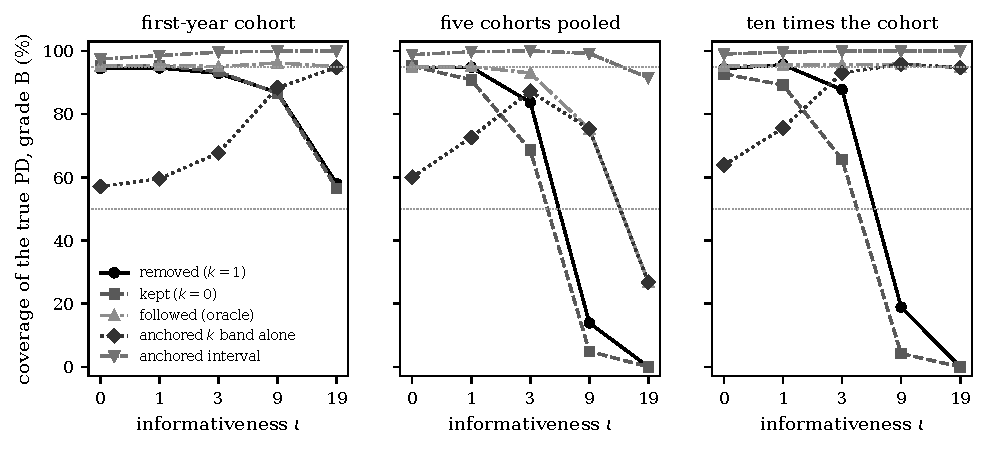
\includegraphics[width=\textwidth]{fig-coverage-k}
\caption{Coverage of grade B's true one-year PD against the informativeness of withdrawal in the generator, for the first annual cohort, the five cohorts pooled and the cohort ten times larger, for removal, keeping, the oracle that follows the \wdn{} ratings, the band of the anchored $k$ alone and the anchored interval; dotted lines mark 95\% and 50\%, 1,000 repetitions per point.}
\label{fig:coverage-k}
\end{figure}

\subsection{Cohort size}

The size of the cohort decides whether a bias can be seen. Table~\ref{tab:scale} and Figure~\ref{fig:scale} raise the first annual cohort from the case's size to thirty times it at informativeness 9. Removal covers \nv{cov.fy.i9.industry}\% at the case's size, \nv{cov.x3.i9.industry}\% at three times, \nv{cov.x10.i9.industry}\% at ten times and \nv{cov.x30.i9.industry}\% at thirty times, as its relative bias of about $-\nv{abias.x30.i9.industry}\%$ stays while its sampling interval shrinks. The oracle covers \nv{cov.x3.i9.followed}\% to \nv{cov.x30.i9.followed}\% throughout, and the anchored interval \nv{cov.x3.i9.anchored}\% to \nv{cov.x30.i9.anchored}\%. The width of the anchored interval shrinks with the cohort, from \nv{w.fy.i9.anchored} to \nv{w.x30.i9.anchored} percentage points, in a ratio to the oracle's width that stays near two; the Manski band hardly shrinks, from \nv{w.fy.i9.identified} to \nv{w.x30.i9.identified}, because its width is set by the share of \wdn{} ratings and not by the number of ratings.

\begin{table}[htbp]
\centering
\footnotesize
\caption{Coverage (\%) of grade B's true one-year PD at informativeness 9 as the cohort grows from the case's size to thirty times it, for the removed, followed and anchored treatments with Monte Carlo standard errors, and the mean widths in percentage points of the anchored interval, the followed interval and the Manski band.}
\label{tab:scale}
\begin{tabular}{llrrrrrr}
\toprule
Cohort & Reps & Removed & Followed & Anchored & $W_{\rm anch}$ & $W_{\rm fol}$ & $W_{\rm Manski}$ \\
\midrule
$\times1$ & 1,000 & $86.8\pm1.1$ & $96.2\pm0.6$ & $99.9\pm0.1$ & 2.16 & 1.13 & 8.26 \\
$\times3$ & 500 & $66.8\pm2.1$ & $96.2\pm0.9$ & $100.0\pm0.0$ & 1.29 & 0.66 & 7.10 \\
$\times10$ & 1,000 & $18.9\pm1.2$ & $95.8\pm0.6$ & $100.0\pm0.0$ & 0.72 & 0.36 & 6.63 \\
$\times30$ & 500 & $0.0\pm0.0$ & $94.2\pm1.0$ & $100.0\pm0.0$ & 0.41 & 0.21 & 6.39 \\
\bottomrule
\end{tabular}
\end{table}


\begin{figure}[htbp]
\centering
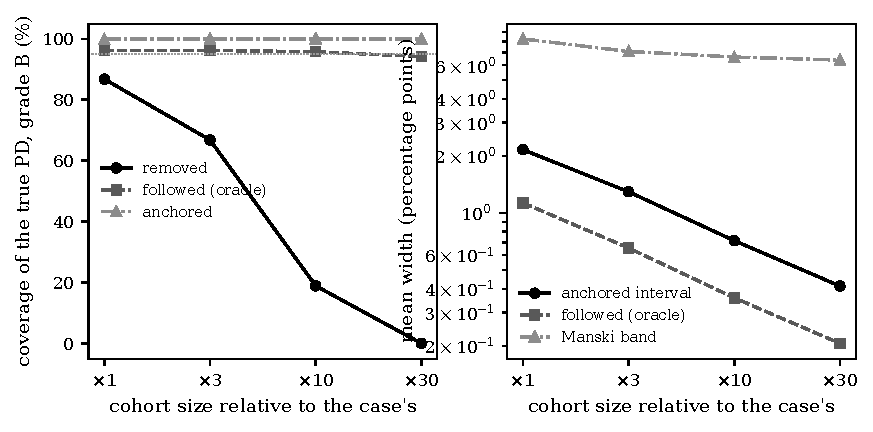
\includegraphics[width=0.9\textwidth]{fig-scale}
\caption{Coverage of grade B's true PD and mean interval width as the first annual cohort grows from the case's size to thirty times it at informativeness 9; left, coverage of removal, the oracle that follows the \wdn{} ratings and the anchored interval; right, the widths of the anchored interval, the oracle's interval and the Manski band on a logarithmic axis.}
\label{fig:scale}
\end{figure}

\subsection{A second source with another definition}

The coverage results above use a second source that counts exactly the followed cohort's defaults. Table~\ref{tab:capture} and Figure~\ref{fig:capture} vary that count at informativeness 9: the second source counts a share $c$ of the defaults, or the defaults and other events. The coverage of the anchored interval is robust: \nv{cap.i9.c0.5.cov}\% at $c=0.5$, \nv{cap.i9.c0.8.cov}\% at 0.8, \nv{cap.i9.c1.1.cov}\% at 1.1 and \nv{cap.i9.c1.3.cov}\% at 1.3, as the interval is wide and always contains the oracle's Jeffreys interval for the count it is given. The centre is not. The relative bias of the anchored point is $\nv{cap.i9.c0.8.bias}\%$ at 0.8, $\nv{cap.i9.c0.9.bias}\%$ at 0.9, $+\nv{cap.i9.c1.1.abias}\%$ at 1.1 and $+\nv{cap.i9.c1.3.abias}\%$ at 1.3, as Proposition~\ref{prop:capture} predicts, and the median anchored odds ratio moves from \nv{cap.i9.c0.8.k} to \nv{cap.i9.c1.3.k} against a realised \nv{ktrue.fy.i9}. A source with a capture of 0.5 or 0.7 returns the odds ratio 0 in the median repetition, because it counts fewer defaults than the transition page already saw, and the point sits at the floor of keeping. The window in which anchoring beats removal on bias is $\nv{rho.fy.i9}<c<\nv{rho.hi.fy.i9}$, which this ladder confirms for $c=1.3$: it is outside the window and has a larger bias than removal's $\nv{bias.fy.i9.industry}\%$. The point $c=0.7$ is also outside it, with a bias of $\nv{cap.i9.c0.7.bias}\%$, which differs from removal's by less than twice their standard errors, so it is at removal's level. At informativeness 3 (the lighter lines of Figure~\ref{fig:capture}) the pattern is the same: the anchored coverage is \nv{cap.i3.c0.5.cov}\% at $c=0.5$ and \nv{cap.i3.c1.3.cov}\% at 1.3, and the bias at 1.3 is $+\nv{cap.i3.c1.3.abias}\%$ against $\nv{bias.fy.i3.industry}\%$ for removal.

\begin{table}[htbp]
\centering
\small
\caption{Grade B at informativeness 9 when the second source counts $c$ times the true defaults (below 1) or counts them and other events at rate $c-1$ (above 1): coverage of the anchored interval with its standard error, coverage of the band alone, mean width, relative bias of the anchored point and the median anchored odds ratio, the realised one being the exact-source row.}
\label{tab:capture}
\begin{tabular}{lrrrrr}
\toprule
Capture $c$ & Anchored (\%) & Band alone (\%) & Width (pp) & Bias (\%) & Median $k$ \\
\midrule
0.5 & $97.5\pm0.5$ & 34.2 & 1.29 & $-25.3$ & 0.0 \\
0.7 & $99.7\pm0.2$ & 71.5 & 1.63 & $-21.8$ & 0.0 \\
0.8 & $99.9\pm0.1$ & 81.1 & 1.82 & $-16.6$ & 1.2 \\
0.9 & $99.8\pm0.1$ & 86.7 & 1.99 & $-9.1$ & 3.2 \\
1 (exact) & $99.9\pm0.1$ & 88.3 & 2.16 & $-0.1$ & 5.2 \\
1.1 & $99.9\pm0.1$ & 87.0 & 2.30 & $+9.5$ & 7.2 \\
1.3 & $97.8\pm0.5$ & 71.8 & 2.56 & $+29.7$ & 12.1 \\
\bottomrule
\end{tabular}
\end{table}


\begin{figure}[htbp]
\centering
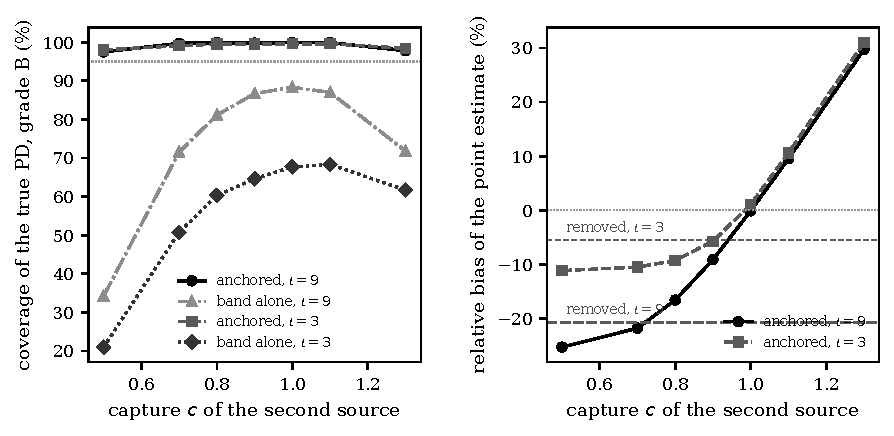
\includegraphics[width=0.95\textwidth]{fig-capture}
\caption{Grade B at informativeness 3 and 9 when the second source counts a share $c$ of the true defaults (below 1) or the defaults and other events (above 1); left, coverage of the anchored interval and of the band alone; right, relative bias of the anchored point, with the bias of removal as horizontal lines; 1,000 repetitions per point.}
\label{fig:capture}
\end{figure}

\subsection{Decisions at a threshold}

A validator uses the PD to decide, so Table~\ref{tab:decisions} and Figure~\ref{fig:decisions} classify each repetition's interval against thresholds set 15 and 30\% below and above the true PD. The removed estimate commits mistakes where the bias runs against the threshold: in the pooled design at informativeness 9 its interval lies wholly below a threshold 15\% under the true PD in \nv{dec.pool.i9.industry.-0.15.w}\% of the repetitions, saying that the PD is below a value it exceeds. The anchored interval never lands on the wrong side in any of the twelve cells of the table, but it is across the threshold in \nv{dec.fy.i9.anchored.-0.15.u}\% of the repetitions at a 15\% offset in the first annual cohort, and in \nv{dec.pool.i9.anchored.-0.15.u}\% when pooled. At ten times the cohort it separates a threshold 30\% below the true PD in \nv{dec.x10.i9.anchored.-0.30.c}\% of the repetitions and one 30\% above in \nv{dec.x10.i9.anchored.+0.30.c}\%. At the case's size the method is silent rather than wrong: the interval tells the validator that the decision cannot be taken from the transition page and one second source.

\begin{table}[htbp]
\centering
\footnotesize
\caption{Threshold decisions on grade B at informativeness 9, for a threshold $t=\mathrm{PD}(1+\delta)$ around the true PD: the percentage of 1,000 repetitions in which the 95\% interval lies on the correct side, on the wrong side, or across the threshold (correct / wrong / undetermined).}
\label{tab:decisions}
\begin{tabular}{llrrrr}
\toprule
Design & Treatment & $\delta=-0.30$ & $\delta=-0.15$ & $\delta=+0.15$ & $\delta=+0.30$ \\
\midrule
first-year cohort & Removed & 6 / 1 / 93 & 1 / 4 / 94 & 25 / 0 / 75 & 45 / 0 / 55 \\
 & Followed (oracle) & 28 / 0 / 72 & 9 / 1 / 90 & 6 / 1 / 93 & 17 / 0 / 83 \\
 & Anchored & 4 / 0 / 96 & 1 / 0 / 99 & 0 / 0 / 100 & 0 / 0 / 100 \\
five cohorts pooled & Removed & 0 / 7 / 93 & 0 / 45 / 55 & 99 / 0 / 1 & 100 / 0 / 0 \\
 & Followed (oracle) & 27 / 0 / 73 & 2 / 3 / 96 & 72 / 0 / 28 & 96 / 0 / 4 \\
 & Anchored & 0 / 0 / 100 & 0 / 0 / 100 & 7 / 0 / 93 & 36 / 0 / 64 \\
ten times the cohort & Removed & 23 / 0 / 77 & 0 / 15 / 85 & 100 / 0 / 0 & 100 / 0 / 0 \\
 & Followed (oracle) & 99 / 0 / 1 & 52 / 0 / 48 & 45 / 0 / 55 & 96 / 0 / 4 \\
 & Anchored & 64 / 0 / 36 & 2 / 0 / 98 & 2 / 0 / 98 & 36 / 0 / 64 \\
\bottomrule
\end{tabular}
\end{table}


\begin{figure}[htbp]
\centering
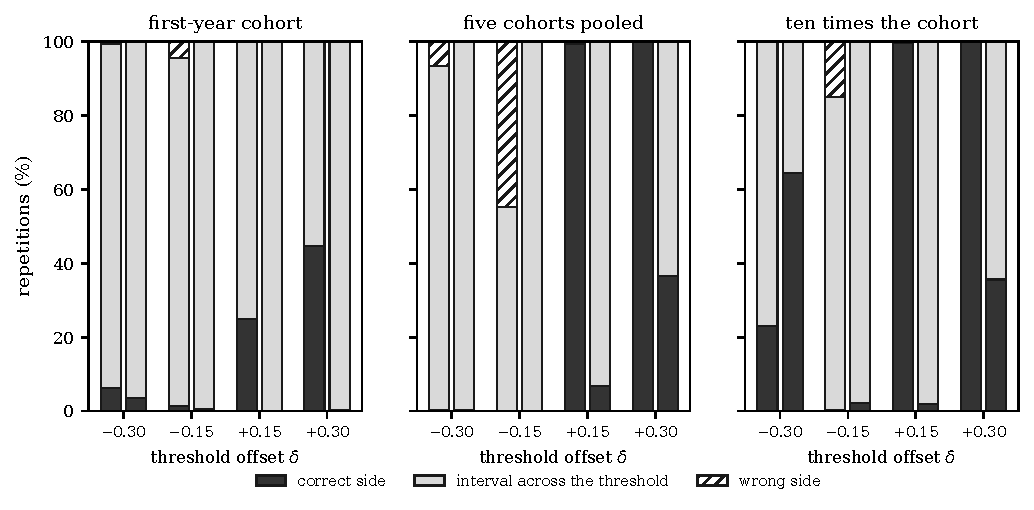
\includegraphics[width=\textwidth]{fig-decisions}
\caption{Threshold decisions on grade B at informativeness 9: for each offset of the threshold from the true PD, the share of 1,000 repetitions in which the interval of the removed estimate (left bar) and of the anchored interval (right bar) lies on the correct side, across the threshold, or on the wrong side, in the three designs.}
\label{fig:decisions}
\end{figure}

\subsection{Agency cohorts}

Table~\ref{tab:real} gives the anchored result on the agencies' cohorts, with the default page as the second source. For S\&P's grade B, pooled over the \nv{real.sp.cohorts} annual cohorts, the transition page counts $D=\nv{real.sp.B.D}$ defaults, $S=\nv{real.sp.B.S}$ survivors and $W=\nv{real.sp.B.W}$ \wdn{} ratings, and the default page counts $A=\nv{real.sp.B.A}$ defaults over $N_a=\nv{real.sp.B.Na}$ ratings. Removal gives a PD of \nv{real.sp.B.pdind}\%; the anchored PD is \nv{real.sp.B.pdanc}\%, with an interval from \nv{real.sp.B.pdlo}\% to \nv{real.sp.B.pdhi}\%. The pooled anchored odds ratio is \nv{real.sp.B.k}, with a band from \nv{real.sp.B.klo} to \nv{real.sp.B.khi}. Figure~\ref{fig:pd-curve} places these on the family: the anchored point lies where the curve has risen to the second source's count, and the tipping $\tip$ to the next grade is \nv{real.sp.B.tip}, a little above the anchored band, so the anchored PD of B does not reach the threshold of \nv{real.sp.B.tipthr}\% that separates it from CCC to C.

\begin{figure}[htbp]
\centering
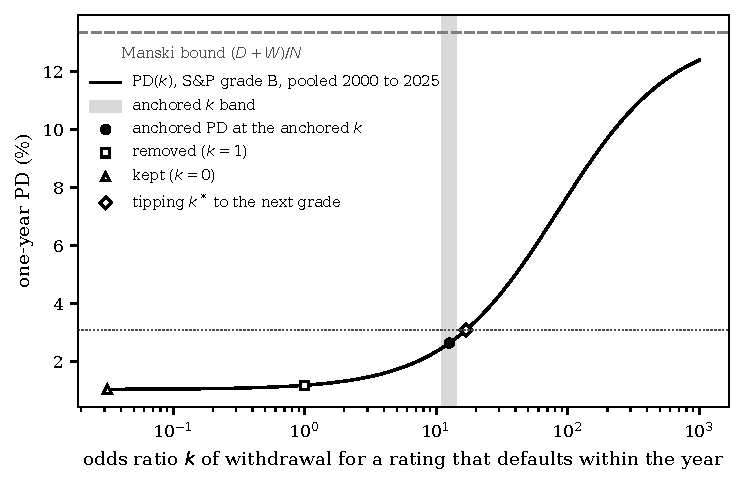
\includegraphics[width=0.85\textwidth]{fig-pd-curve}
\caption{The family PD$(k)$ of S\&P's grade B pooled over all annual cohorts, from the transition page's counts of defaults, survivors and \wdn{} ratings, with the removed estimate, the kept estimate, Manski's bound, the anchored odds ratio with its band and the tipping odds ratio at the threshold to the next grade.}
\label{fig:pd-curve}
\end{figure}

\begin{table}[htbp]
\centering
\footnotesize
\caption{Anchored withdrawal bounds on the agencies' real cohorts of ESMA's central repository, the default page as the second source of the transition page: the pooled PD with withdrawals removed, the anchored PD with its interval, the pooled anchored odds ratio with its band, the cohorts whose band contains it, and the tipping odds ratio that moves the grade to the next one.}
\label{tab:real}
\begin{tabular}{llrp{2.4cm}p{2.6cm}rr}
\toprule
Agency & Grade & PD removed (\%) & Anchored PD (\%) & Pooled $k$ (band) & Cohorts holding it & Tipping $k$ \\
\midrule
S\&P & AA & 0.00 & 0.01 (0.00 to 0.06) & 17.2 (0.0 to 93.6) & 1 of 1 & 26.8 \\
 & A & 0.03 & 0.03 (0.02 to 0.08) & 5.0 (0.0 to 20.7) & 4 of 4 & 16.5 \\
 & BBB & 0.08 & 0.12 (0.06 to 0.19) & 7.9 (2.3 to 15.0) & 8 of 9 & 18.6 \\
 & BB & 0.35 & 0.55 (0.39 to 0.74) & 7.5 (4.9 to 10.5) & 14 of 16 & 10.3 \\
 & B & 1.17 & 2.63 (2.31 to 2.97) & 12.6 (11.2 to 14.1) & 17 of 25 & 16.8 \\
 & CCC to C & 8.07 & 27.43 (25.08 to 29.87) & 36.3 (29.2 to 46.4) & 16 of 25 & -- \\
Fitch & BBB & 0.01 & 0.08 (0.03 to 0.17) & 139.3 (80.1 to 223.3) & 1 of 2 & 35.9 \\
 & BB & 0.15 & 0.44 (0.24 to 0.74) & 24.7 (15.4 to 36.6) & 8 of 8 & 11.6 \\
 & B & 0.52 & 2.09 (1.53 to 2.75) & 31.6 (25.3 to 39.1) & 7 of 10 & 18.4 \\
 & CCC to C & 4.07 & 22.16 (18.02 to 26.69) & 61.2 (42.7 to 96.6) & 11 of 12 & -- \\
\bottomrule
\end{tabular}
\end{table}


For S\&P's CCC to C grade, the pooled anchored odds ratio is \nv{real.sp.CCC-C.k} with a band from \nv{real.sp.CCC-C.klo} to \nv{real.sp.CCC-C.khi}, and the anchored PD \nv{real.sp.CCC-C.pdanc}\% against \nv{real.sp.CCC-C.pdind}\% for removal. In the other grades of S\&P the pooled anchored $k$ is \nv{real.sp.AA.k} for AA, \nv{real.sp.A.k} for A, \nv{real.sp.BBB.k} for BBB, \nv{real.sp.BB.k} for BB and \nv{real.sp.B.k} for B, all above 1. The tipping $k$ is where the agencies differ, as Figure~\ref{fig:tipping} shows for every grade: the anchored $k$ of every S\&P grade lies to the left of the diamond, and that of Fitch's grades BBB, BB and B to its right. For S\&P the pooled anchored $k$ is below the tipping $k$ of every grade that has one, for example \nv{real.sp.BB.k} against \nv{real.sp.BB.tip} for BB, and only the upper end of the band reaches it, in grades AA, A and BB, where the band of grade BB ends at \nv{real.sp.BB.khi}. For Fitch the anchored $k$ is above the tipping $k$ in grades BBB, BB and B, so the anchored PD of each lies beyond the next notch: for BB, $\widehat k=\nv{real.fitch.BB.k}$ against $\tip=\nv{real.fitch.BB.tip}$. The default categories of Fitch's transition pages hold no rating in \nv{fitch.empty.n} of its \nv{real.fitch.cohorts} years, \nv{fitch.empty.first} to \nv{fitch.empty.last}, while its default page counts \nv{fitch.empty.lost} defaulted ratings in them; those ratings sit among the \wdn{} ones, so the anchored $k$ of Fitch measures the definition of its transition page as much as informative withdrawal.

Figure~\ref{fig:forest} shows the annual anchored $k$ with its band for S\&P's grades B and CCC to C and for Fitch's grade B, against the pooled value. The annual values range widely and the bands are wide, which is a sampling effect, but for the two S\&P grades the pooled value lies outside the annual band in a third of the years.

\begin{figure}[htbp]
\centering
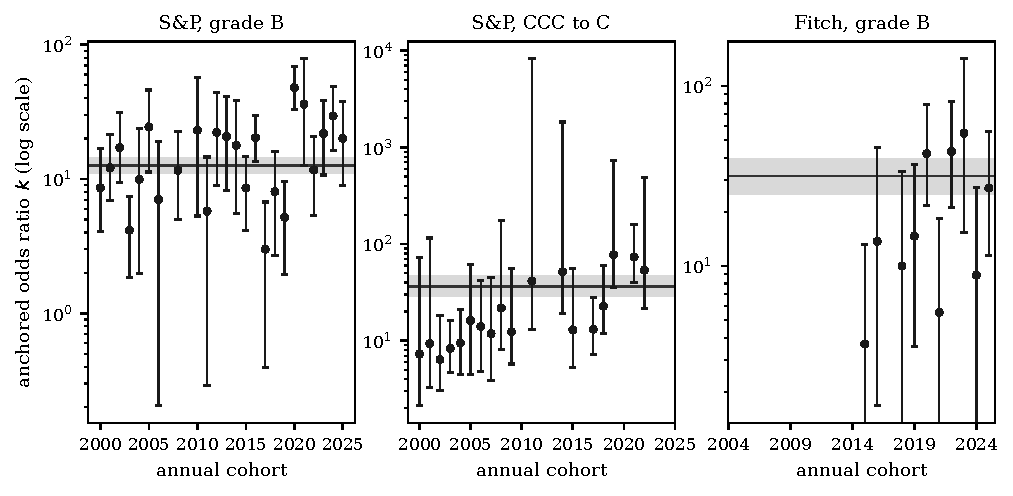
\includegraphics[width=\textwidth]{fig-forest}
\caption{Anchored odds ratio $k$ of each annual cohort with its band, on a logarithmic axis, for S\&P grade B, S\&P grade CCC to C and Fitch grade B, against the pooled anchored odds ratio and its band (horizontal line and shaded area); the default page of the repository is the second source.}
\label{fig:forest}
\end{figure}

\begin{figure}[htbp]
\centering
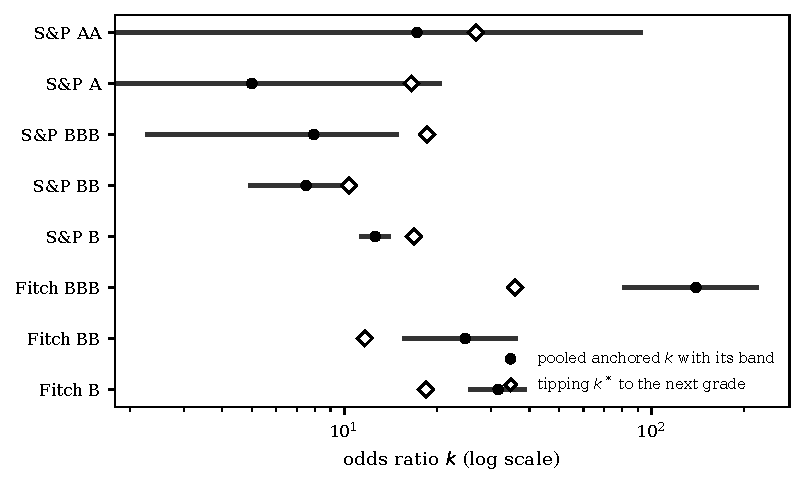
\includegraphics[width=0.85\textwidth]{fig-tipping}
\caption{Pooled anchored odds ratio with its band (circle and segment) and tipping odds ratio to the next grade (diamond), on a logarithmic axis, for each grade of S\&P and Fitch that has an anchored value; where the band lies to the right of the diamond the anchored PD is beyond the next notch of the scale.}
\label{fig:tipping}
\end{figure}

\subsection{Stability of the anchored odds ratio}

The criterion of Equation~\eqref{eq:stability} fails for the agencies' cohorts: \nv{real.sp.B.contain} of \nv{real.sp.B.usable} annual cohorts of S\&P's grade B hold the pooled $k$ in their band, \nv{real.sp.B.share}\%, and \nv{real.sp.CCC-C.contain} of \nv{real.sp.CCC-C.usable} of CCC to C, \nv{real.sp.CCC-C.share}\%; grades BB and BBB of S\&P pass with \nv{real.sp.BB.share}\% and \nv{real.sp.BBB.share}\%. For Fitch, grade B has \nv{real.fitch.B.contain} of \nv{real.fitch.B.usable} and grade BBB \nv{real.fitch.BBB.contain} of \nv{real.fitch.BBB.usable}, on two usable cohorts only. Table~\ref{tab:stability} and Figure~\ref{fig:stability} ask where that instability can come from, by applying the same criterion on known truth. With an exact second source the share of cohorts that hold the pooled $k$ is \nv{stab.i9.c1.B.share}\% in grade B at informativeness 9 and \nv{stab.i3.c1.B.share}\% at 3, so sampling noise alone does not produce it. A second source that counts a constant multiple of the defaults gives \nv{stab.i9.c1.3.B.share}\% at 9 (the series at 1.3 times of Figure~\ref{fig:stability}), and one whose multiple is drawn each year from 1.0 to 1.6 gives \nv{stab.i9.cu1.0-1.6.B.share}\%. When the multiple is drawn each year from 1.0 to 4.0, the share falls to \nv{stab.i9.cu1.0-4.0.B.share}\% for grade B, \nv{stab.i9.cu1.0-4.0.BB.share}\% for BB and \nv{stab.i9.cu1.0-4.0.CCC-C.share}\% for CCC to C (at informativeness 3, \nv{stab.i3.cu1.0-4.0.B.share}\% for grade B).

These multiples scale the followed count $D+X$, not the count $D$ of the transition page, so they are not on the scale of the ratio observed on the agency data. That ratio, the default page's rate over the transition page's rate, $(A/N_a)/(D/N)$, runs for S\&P's grade B over its \nv{ratio.B.n} cohorts with defaults from \nv{ratio.B.min} to \nv{ratio.B.max}, with a median of \nv{ratio.B.median}, a mean of \nv{ratio.B.mean} and \nv{ratio.B.above4} cohorts above 4.0; for CCC to C over \nv{ratio.CCC-C.n} cohorts from \nv{ratio.CCC-C.min} to \nv{ratio.CCC-C.max}, with a median of \nv{ratio.CCC-C.median}, a mean of \nv{ratio.CCC-C.mean} and \nv{ratio.CCC-C.above4} cohorts above 4.0; and for BB over \nv{ratio.BB.n} cohorts from \nv{ratio.BB.min} to \nv{ratio.BB.max}, with a median of \nv{ratio.BB.median}. The range of 1.0 to 4.0 is therefore a variation from year to year of the same order, not a matched one. The last series draws each year, for each grade, a multiple of the defaults $D$ that the transition page observes, uniformly between the extremes of that grade's own observed ratio. It is a draw over the observed range and not a resampling of the observed ratios, and it is centred higher than they are: its mean and median are \nv{ratio.B.draw.mean} for grade B against an observed mean of \nv{ratio.B.mean} and median of \nv{ratio.B.median}, with \nv{ratio.B.draw.above4}\% of its mass above 4.0 against \nv{ratio.B.above4} of \nv{ratio.B.n} cohorts, and \nv{ratio.CCC-C.draw.mean} for CCC to C against \nv{ratio.CCC-C.mean} and \nv{ratio.CCC-C.median}. Under it the share of cohorts that hold the pooled $k$ is, at informativeness 9, \nv{stab.i9.cdobs.B.share}\% for grade B against \nv{real.sp.B.share}\% observed, \nv{stab.i9.cdobs.BB.share}\% for BB against \nv{real.sp.BB.share}\%, and \nv{stab.i9.cdobs.CCC-C.share}\% for CCC to C against \nv{real.sp.CCC-C.share}\%; \nv{stab.i9.cdobs.B.stable}\%, \nv{stab.i9.cdobs.BB.stable}\% and \nv{stab.i9.cdobs.CCC-C.stable}\% of the repetitions of the three grades reach the 80\% criterion. The CCC to C figures are over the \nv{stab.i9.cdobs.CCC-C.defined} repetitions at informativeness 9 (\nv{stab.i3.cdobs.CCC-C.defined} at 3) in which a share is defined, and at informativeness 3 the pooled $k$ of CCC to C is infinite in every repetition. The level of the draw is also above the observed one: the median pooled $k$ of grade B is \nv{stab.i9.cdobs.B.k} against the \nv{real.sp.B.k} observed. A definition gap that varies by year over the range observed for grade B therefore brings its share near the observed one, although the draw is centred above the observed ratios; the same study over the range observed for CCC to C leaves its share above the observed one and does not make it fail, and the gap does not make BB fail, as the observed BB does not. The instability of the anchored $k$ for grade B has the size that a year-to-year change in the definition gap produces and not the size that sampling produces; that this change is its cause is not shown, and what makes the anchored $k$ of CCC to C unstable is not explained by this study (Section~\ref{sec:limitations}).

\begin{table}[htbp]
\centering
\footnotesize
\caption{Stability criterion on known truth: over 1,000 repetitions of five annual cohorts, the mean share of cohorts whose anchored $k$ band contains the pooled anchored $k$ with its standard error, the share of repetitions that reach the 80\% criterion, and the median pooled anchored $k$, at informativeness 3 (panel a) and 9 (panel b) for five second sources: exact; counting 1.3 times the defaults every year; a multiple of the defaults drawn each year from 1.0 to 1.6 and from 1.0 to 4.0; and a multiple of the defaults the transition page observes drawn each year from the range of the grade's own observed ratio of the default page's rate to the transition page's rate, uniform on 0.97 to 5.00 for BB, 1.62 to 7.00 for B and 2.05 to 9.81 for CCC to C. A dash is a median pooled $k$ that is undefined: the pooled $k$ is infinite in every repetition, because the second source counts more defaults than the cohorts' defaults and withdrawals together. Where fewer than 1,000 repetitions have a share (a grade without a usable cohort), the figures are over the repetitions defined: 367 at fewest.}
\label{tab:stability}
\textbf{(a) Informativeness $\iota=3$}\par\smallskip
\begin{tabular}{p{4.2cm}lp{2.4cm}p{2.0cm}r}
\toprule
Capture & Grade & Cohorts holding pooled $k$ (\%) & Repetitions stable (\%) & Median pooled $k$ \\
\midrule
exact & BB & $100.0\pm0.0$ & 99.9 & 1.8 \\
 & B & $100.0\pm0.0$ & 100.0 & 2.2 \\
 & CCC to C & $100.0\pm0.0$ & 100.0 & 1.8 \\
1.3 times & BB & $99.8\pm0.1$ & 99.5 & 7.5 \\
 & B & $99.7\pm0.1$ & 100.0 & 8.0 \\
 & CCC to C & $99.9\pm0.0$ & 100.0 & 11.4 \\
1.0 to 1.6 by year & BB & $99.4\pm0.1$ & 99.2 & 7.3 \\
 & B & $98.7\pm0.2$ & 99.6 & 8.0 \\
 & CCC to C & $97.9\pm0.2$ & 99.4 & 11.2 \\
1.0 to 4.0 by year & BB & $90.4\pm0.5$ & 83.3 & 31.0 \\
 & B & $64.5\pm0.7$ & 39.4 & 40.8 \\
 & CCC to C & $82.0\pm0.9$ & 63.1 & 72.6 \\
observed ratio range of the grade, by year & BB & $93.5\pm0.4$ & 89.4 & 34.6 \\
 & B & $53.8\pm0.7$ & 21.1 & 111.3 \\
 & CCC to C & $99.2\pm0.4$ & 98.9 & -- \\
\bottomrule
\end{tabular}
\medskip

\textbf{(b) Informativeness $\iota=9$}\par\smallskip
\begin{tabular}{p{4.2cm}lp{2.4cm}p{2.0cm}r}
\toprule
Capture & Grade & Cohorts holding pooled $k$ (\%) & Repetitions stable (\%) & Median pooled $k$ \\
\midrule
exact & BB & $99.8\pm0.1$ & 99.8 & 5.8 \\
 & B & $99.5\pm0.1$ & 100.0 & 5.8 \\
 & CCC to C & $99.8\pm0.1$ & 100.0 & 4.4 \\
1.3 times & BB & $99.0\pm0.2$ & 98.4 & 12.5 \\
 & B & $98.2\pm0.2$ & 99.6 & 12.8 \\
 & CCC to C & $99.3\pm0.1$ & 100.0 & 14.1 \\
1.0 to 1.6 by year & BB & $98.4\pm0.2$ & 97.3 & 12.6 \\
 & B & $96.6\pm0.3$ & 98.6 & 12.9 \\
 & CCC to C & $97.2\pm0.2$ & 99.5 & 13.8 \\
1.0 to 4.0 by year & BB & $86.9\pm0.6$ & 72.5 & 42.1 \\
 & B & $64.7\pm0.7$ & 41.1 & 49.8 \\
 & CCC to C & $76.2\pm0.9$ & 48.2 & 103.2 \\
observed ratio range of the grade, by year & BB & $97.2\pm0.3$ & 95.6 & 33.6 \\
 & B & $61.2\pm0.7$ & 33.5 & 76.2 \\
 & CCC to C & $89.7\pm0.9$ & 83.9 & 221.4 \\
\bottomrule
\end{tabular}
\end{table}


\begin{figure}[htbp]
\centering
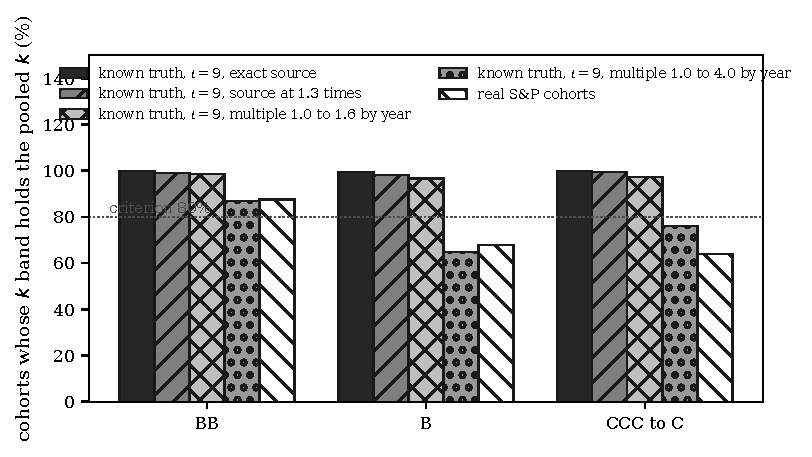
\includegraphics[width=0.85\textwidth]{fig-stability}
\caption{Share of annual cohorts whose anchored $k$ band contains the pooled anchored $k$, by grade: on known truth at informativeness 9 with an exact second source, a second source at 1.3 times the defaults, a multiple of the defaults drawn each year from 1.0 to 1.6 and from 1.0 to 4.0, and a multiple of the observed defaults drawn each year over the range of the grade's own observed ratio, and on the real cohorts of S\&P; the dotted line is the 80\% criterion.}
\label{fig:stability}
\end{figure}

\subsection{Outcome of each prediction}

Table~\ref{tab:hypotheses} sets the predictions of Section~\ref{sec:experimental-design} against the measurements. H1 holds: the anchored interval covers between \nv{h1.min}\% and 100\% of the repetitions at informativeness 1, 3 and 9 in the first-year, pooled and ten-fold designs (the product's criterion reads the ten-fold design at 9 only; at 1 and 3 it gives \nv{cov.x10.i1.anchored}\% and \nv{cov.x10.i3.anchored}\%). In the first-year and ten-fold designs Proposition~\ref{prop:containment} makes this certain for an exact second source; in the pooled design it is an empirical result. H2 holds for removal and keeping only where the bias outgrows the noise, in the pooled and ten-fold designs, and fails in the first annual cohort, where they cover \nv{cov.fy.i9.industry}\% and \nv{cov.fy.i9.unfollowed}\%; the oracle that follows the \wdn{} ratings, which the product reports apart, is under 50\% in none of the three designs.

H3 fails as worded. Against the removed, kept and followed treatments, the comparison of the product's committed criterion, it holds in all three designs, by margins of \nv{h3.single.fy}, \nv{h3.single.pool} and \nv{h3.single.x10} points. Against the Manski band, a published treatment run on the same draws, the anchored interval does not cover more often: the difference in coverage is \nv{h3.man.fy} points in the first annual cohort, \nv{h3.man.pool} points in the pooled design, where the band covers \nv{cov.pool.i9.identified}\% against \nv{cov.pool.i9.anchored}\% and the gap exceeds twice the larger standard error, and \nv{h3.man.x10} points in the ten-fold cohort. What the anchored interval buys against the band is width and not coverage: at informativeness 9 it is \nv{wr.fy.i9}, \nv{wr.pool.i9} and \nv{wr.x10.i9} times narrower than the band in the three designs (\nv{w.fy.i9.anchored} against \nv{w.fy.i9.identified}, \nv{w.pool.i9.anchored} against \nv{w.pool.i9.identified} and \nv{w.x10.i9.anchored} against \nv{w.x10.i9.identified} percentage points). H4 fails: the anchored $k$ of the agencies' grades B and CCC to C is not stable across years, and the instability of grade B has the size of a definition gap that varies by year. H5 holds, with a pooled $k$ of \nv{real.sp.CCC-C.k} and a lower band limit of \nv{real.sp.CCC-C.klo}, both above 1.

The prediction as a whole is refuted. Its refutation clause reads that it is refuted if the anchored interval does not cover more than the existing treatments or if the anchored odds ratio is unstable across years. Both refutation conditions are met: the anchored odds ratio is unstable across years on the agencies' data (H4), and the anchored interval does not cover more than the Manski band (H3). On known truth the coverage clauses hold against the single-answer treatments, and the clause that every existing treatment falls under 50\% holds only for removal and keeping where the cohort is large enough.

\begin{table}[htbp]
\centering
\small
\caption{The predictions stated before the experiments and their outcome: the quantity each measures, the value measured in the first-year, pooled and ten-fold designs (in that order where three are given), the criterion, and whether it held at the repetitions of the grid.}
\label{tab:hypotheses}
\begin{tabular}{lp{4.6cm}p{4.2cm}p{1.8cm}p{2.4cm}}
\toprule
Id & Quantity & Measured (\%, or $k$) & Criterion & Outcome \\
\midrule
H1 & \relax anchored coverage at $\iota=1,3,9$ & 98.5 to 100.0 & at least 90 & holds \\
H2 & \relax removed and kept coverage at $\iota=9$ & first-year cohort 87/87; five cohorts pooled 14/5; ten times the cohort 19/4 & under 50 & holds in two of three designs \\
H2' & \relax followed (oracle) coverage at $\iota=9$ & 96; 75; 96 & under 50 & fails in all three \\
H3 & \relax anchored minus best existing coverage at $\iota=9$ & +3.7; +23.9; +4.2 & above 0 & holds \\
H4 & \relax share of cohorts whose band holds the pooled $k$, S\&P grade B and CCC to C & 68; 64 & at least 80 & fails \\
H5 & \relax pooled anchored $k$ of CCC to C, S\&P & 36.3 & above 1 & holds \\
\bottomrule
\end{tabular}
\end{table}

